\documentclass[12pt]{scrartcl}

\usepackage[utf8]{inputenc}
\usepackage[T1]{fontenc}
\usepackage{lmodern}
\usepackage{graphicx}
%\usepackage[pdftex,hyperref,dvipsnames]{xcolor}
\usepackage{listings}
\usepackage[a4paper,lmargin={2cm},rmargin={2cm},tmargin={3.5cm},bmargin = {2.5cm},headheight = {4cm}]{geometry}
\usepackage{amsmath,amssymb,amstext,amsthm}
% \usepackage[lined,algonl,boxed]{algorithm2e} 
%\usepackage{algpseudocode}
\usepackage{tikz}
\usepackage{pgfplots}
\usepackage{url}
\usepackage{tcolorbox}
\usepackage[inline]{enumitem}
\usepackage[headsepline]{scrlayer-scrpage} 
\usepackage{float}

\usepackage[scale=0.55, lineVdist=1em]{secstack}
\pagestyle{scrheadings} 
\usetikzlibrary{automata,positioning}
\graphicspath{ {./images/} }

\usepgfplotslibrary{external}
%\tikzexternalize
\pgfplotsset{width=10cm,compat=1.9}
\pgfplotsset{every axis/.style={
    axis line style = thick,
    grid = both,
    tick pos = left,
    tick align = outside,
    tick style = {thick,black},
    fill = blue,
	line width = 2pt,
}}

\lstset{
  basicstyle=\ttfamily\small,
  numbers=left,
  numberstyle=\tiny,
  stepnumber=1,
  numbersep=8pt,
  frame=single,
  breaklines=true,
  columns=fullflexible
}

\lstset{
  language=C,
  basicstyle=\ttfamily\small,
  keywordstyle=\color{blue},
  commentstyle=\color{gray},
  stringstyle=\color{green!60!black},
  numbers=left,
  numberstyle=\tiny,
  stepnumber=1,
  numbersep=8pt,
  frame=single,
  breaklines=true,
  columns=fullflexible
}

\renewcommand{\theenumi}{(\alph{enumi})}
\renewcommand{\labelenumi}{\text{\theenumi}}
\renewcommand{\labelenumii}{(\roman{enumii})} 

\ohead{Marvin Simon (3883376)\\
       Jan Theil (3794698)}

\ihead{System and Web Security}

\newcounter{exnum}
\newcommand{\exercise}[1]{\section*{Problem \theexnum\stepcounter{exnum}: #1}}

\begin{document}

\setcounter{exnum}{2}
\exercise{Static Code Analysis}

\setcounter{exnum}{3}
\exercise{Return-to-libc}

The main idea for this attack was to overwrite the return address of \texttt{foo()} such that the libc function \texttt{system} is called.
First, let's have a look at the program we want to attack (see exercise sheet for the code):

\begin{itemize}
      \item The address to \texttt{system} is printed out for us.
      \item It also prints the pointers to the addresses of the input parameters.
      \item \texttt{foo} is only called, when \texttt{argc == 2}. Hence, we can only provide a single input string for this attack.
      \item \texttt{foo} copies \texttt{src} (coming from \texttt{argv}) into its local \texttt{buffer}.
\end{itemize}

In order to run this return to libc attack we have to do the following:
\begin{itemize}
      \item Find out the address of \texttt{system} by executing the program: \textit{Address of system: 0x8048314}.
      \item Construct an input string, which overflows \texttt{foo}'s buffer, such that
            \begin{itemize}
                  \item \texttt{buffer} is overwritten (8 bytes)
                  \item Old FP is overwritten (4 bytes)
                  \item Ret is replaced by address to \texttt{system} (4 bytes)
                  \item Some dummy ret for \texttt{system} call is inserted (4 bytes)
                  \item Pointer to some string that contains \textit{/bin/sh} (4 bytes)
            \end{itemize}
\end{itemize}

Below is a visualization of how this attack works.

A function call to \texttt{foo} might look like this:\\
\stackLine[24]{C1C}
\stackVariable[8]{C1C}{buffer}
\stackVariable{C24}{old FP}
\stackVariable{C28}{ret}

By overflowing \texttt{buffer} we construct this:\\
\stackLine[24]{C1C}
\stackVariable[1]{C1C}{/}
\stackVariable[1]{C1D}{b}
\stackVariable[1]{C1e}{i}
\stackVariable[1]{C1f}{n}
\stackVariable[1]{C20}{/}
\stackVariable[1]{C21}{s}
\stackVariable[1]{C22}{h}
\stackVariable[1]{C23}{;}
\stackVariable{C24}{*}
\stackVariable{C28}{system}
\stackVariable{C2C}{dummy ret}
\stackVariable{C30}{0xc1c}

So we basically pass the attack string itself as argument to the \texttt{system} call. Since this string
starts with \textit{/bin/sh} it will start a shell.\\

To construct such a string, we have implemented \textit{attack3.c}. This program creates a
string which is 24 bytes long (sum of list above). This string starts with
\textit{/bin/sh;}. This should later be used by \texttt{system} to open a shell.
The bytes 12 - 16 are filled up in little endian format with the address to \texttt{system}.
This is aligned with the former return pointer of \texttt{foo}. Bytes 16 - 20 are some dummy
values for the dummy return and the last 4 bytes are (in the first run) also some dummy values.
We will see shortly why.

As a first step we executed \texttt{./attack3 0x8048314 0x41414141}. This writes the string
\begin{lstlisting}
\x2f\x62\x69\x6e\x2f\x73\x68\x3b\x41\x41\x41\x41\x14\x83\x04\x08\x41\x41\x41\x41\x41\x41\x41\x41
\end{lstlisting}
to a file. Executing the attack program with this string (using \texttt{echo -e '...'}) gives us the
pointer to the input string:

\begin{lstlisting}
Address of system: 0x8048314                                               
Address of argument 0: 0xbffff9ad                                          
Address of argument 1: 0xbffff9c5 <- This is the pointer we will use next
\end{lstlisting}

Replacing the dummy address in the \textit{attack3} call with this address: \texttt{./attack3 0x8048314 0xbffff9c5} results
in
\begin{lstlisting}
\x2f\x62\x69\x6e\x2f\x73\x68\x3b\x41\x41\x41\x41\x14\x83\x04\x08\x41\x41\x41\x41\xc5\xf9\xff\xbf
\end{lstlisting}

Executing \textit{rtlc-exploit-1-target} with this string opens a shell:

\begin{figure}[H]
    \centering
    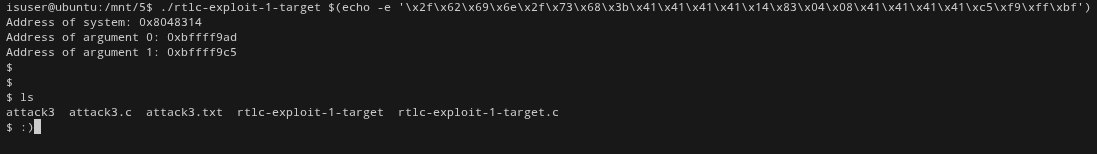
\includegraphics[width=\textwidth]{attack3.png}
    \label{fig:attack3}
\end{figure}

\end{document}
